\documentclass[12pt]{article}
\usepackage[english]{babel}
\usepackage[utf8x]{inputenc}
\usepackage{amsmath}
\usepackage{tikz}
\usetikzlibrary{arrows,automata}
\begin{document}

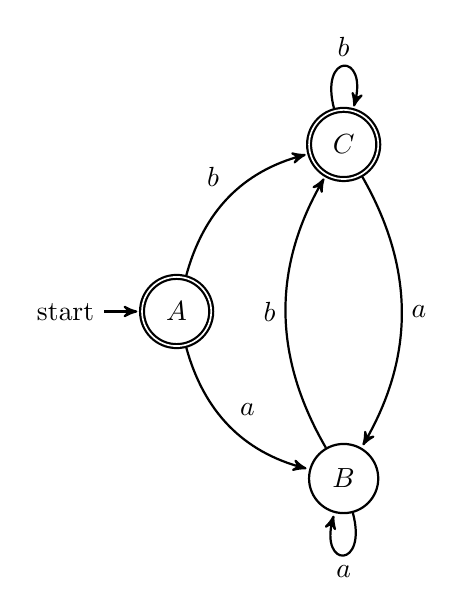
\begin{tikzpicture}[->,>=stealth',shorten >=1pt,auto,node distance=3cm,
    thick,base node/.style={circle,draw,minimum size=8pt}, real node/.style={double,circle,draw,minimum size=17pt}]

  \node[state,initial,accepting]          (a) {$A$};
  \node[state]                  (b) [below right of=a] {$B$};
  \node[state,accepting]        (c)  [above right of = a] {$C$};
  \path (a) edge  [bend right]     node {$a$} (b)
        (a) edge  [bend left]     node {$b$} (c)
        (c) edge  [bend left]     node {$a$} (b)
        (c) edge  [loop above]    node {$b$} (c)
        (b) edge  [loop below]    node {$a$} (b)
        (b) edge  [bend left]     node {$b$} (c)
         ;

\end{tikzpicture}
\end{document}